\documentclass{beamer}
\usetheme{Boadilla}
\usepackage[polish]{babel}
\usepackage[utf8]{inputenc}
\usepackage[T1]{fontenc}
\usepackage{listings}
\usepackage[makeroom]{cancel}

\begin{document}
\title{Chaos Deterministyczny} 
\author{Przemysław Czechowski} 
\date{\today} 

\frame{\titlepage} 

\begin{frame}[fragile]
Problem dwóch ciał?\pause
\begin{lstlisting}
./play.py two_bodies
\end{lstlisting}
\end{frame}

\begin{frame}[fragile]
Problem trzech ciał?\pause
\begin{lstlisting}
./play.py threeA
./play.py threeB
./play.py threeC
\end{lstlisting}
\end{frame}

\begin{frame}{Stabilność układu słonecznego}\pause
\begin{itemize}
\item Czy ziemia zostanie wystrzelona?\pause
\item Czy ziemia może zderzyć się z inną planetą?\pause
\item Jeśli tak, to kiedy?\pause
\end{itemize} 

1887 - nagroda Króla Szwecji: rozwiązać problem N ciał oddziałujących grawitacyjnie\pause\\
Henri Poincaré zdobywa nagrodę, chociaż nie rozwiązał problemu\\
\pause
\centering
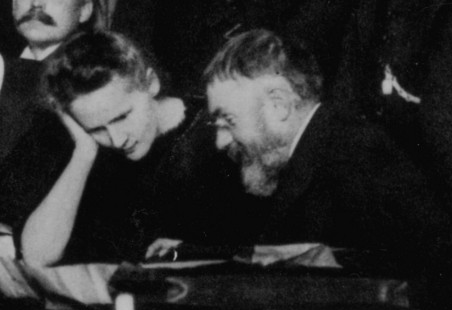
\includegraphics[height=0.4\textheight]{poincare_curie}
\end{frame}

\begin{frame}{Chaos (wg. Royal Society, 1987)}
\pause
\textbf{ Stochastyczne zachowanie występujące w układzie deterministycznym}\pause

Przykłady:\pause
\begin{itemize}[<+->]
\item Problem >2 ciał
\item Przewidywanie pogody
\item Przepływ turbulentny
\item Wzrost niestabilny
	\begin{itemize}[<+->]
		\item Palce lepkości
		\item Wzrost sieci rzecznej
		\item Spalanie papieru w wąskiej szczelinie
	\end{itemize} 
\end{itemize} 
\end{frame}

\begin{frame}{Palce lepkości}
\centering
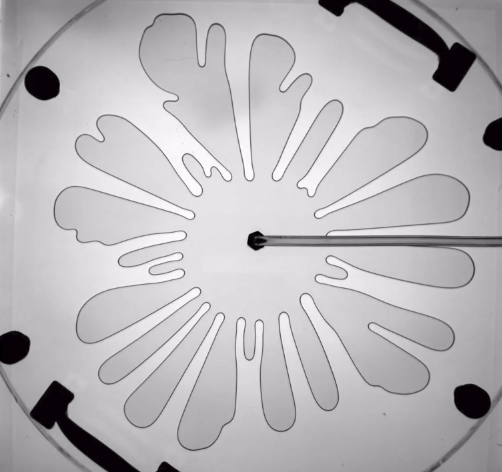
\includegraphics[height=0.6\textheight]{viscous_fingers}
\url{https://www.youtube.com/watch?v=BgeKR9HuY9s}

\end{frame}

\begin{frame}[fragile]
\textbf{Stochastyczne zachowanie występujące w układzie deterministycznym}
\begin{lstlisting}
./play.py butterfly
\end{lstlisting}
\end{frame}

\begin{frame}[t]{Wykładniki Lyapunowa - teoria}
\begin{equation*}
| \delta\mathbf{x}(t) | \approx e^{\lambda t} | \delta \mathbf{x}(0) |
\end{equation*}
\end{frame}

\begin{frame}[t]{Wykładniki Lyapunowa - praktyka}
\begin{equation*}
| \delta\mathbf{x}(t) | \approx e^{\lambda t} | \delta \mathbf{x}(0) |
\end{equation*}
\centering
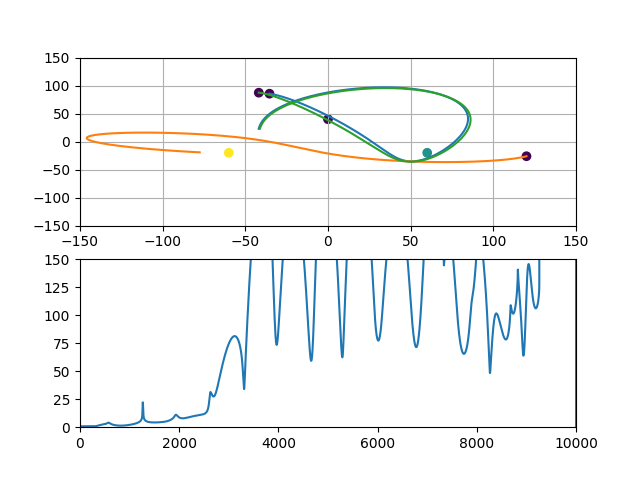
\includegraphics[height=0.7\textheight]{lyapunov}
\end{frame}

\begin{frame}[t]{Wykładniki Lyapunowa - praktyka}
\begin{equation*}
| \delta\mathbf{x}(t) | \approx e^{\lambda t} | \delta \mathbf{x}(0) |
\end{equation*}
\centering
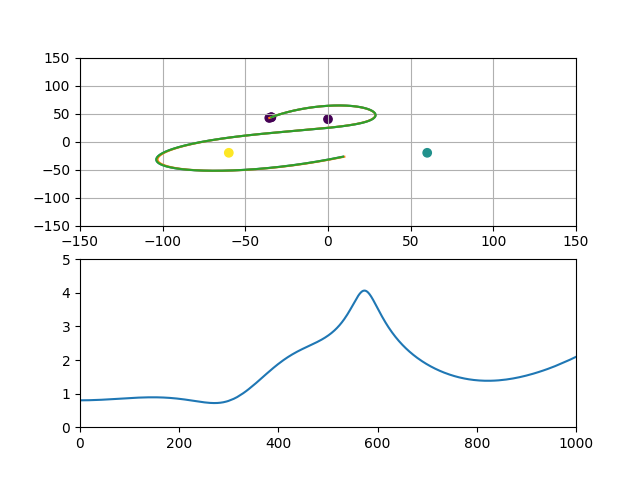
\includegraphics[height=0.7\textheight]{lyapunov_short}
\end{frame}

\begin{frame}[t]{Wykładniki Lyapunowa - praktyka}
\begin{equation*}
| \delta\mathbf{x}(t) | \approx e^{\lambda t} | \delta \mathbf{x}(0) |
\end{equation*}
\centering
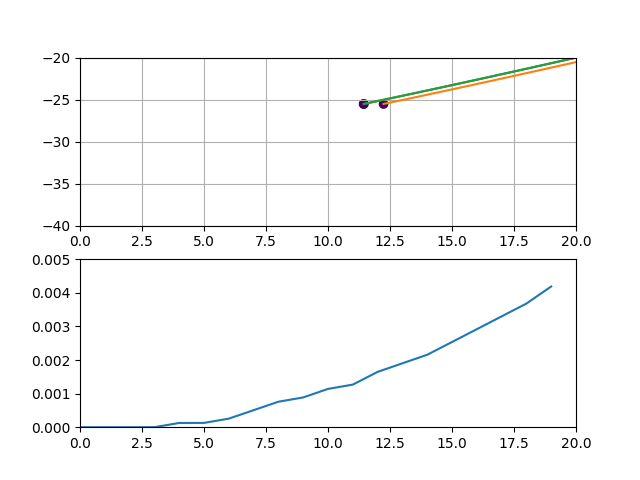
\includegraphics[height=0.7\textheight]{lyapunov_very_short}
\end{frame}

\begin{frame}{Alternatywa dla wykładników Lyapunowa} \pause
\begin{itemize}
	\item Etropia metryczna
	\item Etropia topologiczna
\end{itemize} 
Wymagają innego opisu
\end{frame}

\begin{frame}{Przepływ zamiast równań} \pause
\centering
\begin{equation*}
\xcancel{\dot{x}=y, \dot{y}=\sin{x}}
\end{equation*}
\begin{equation*}
\downarrow
\end{equation*}
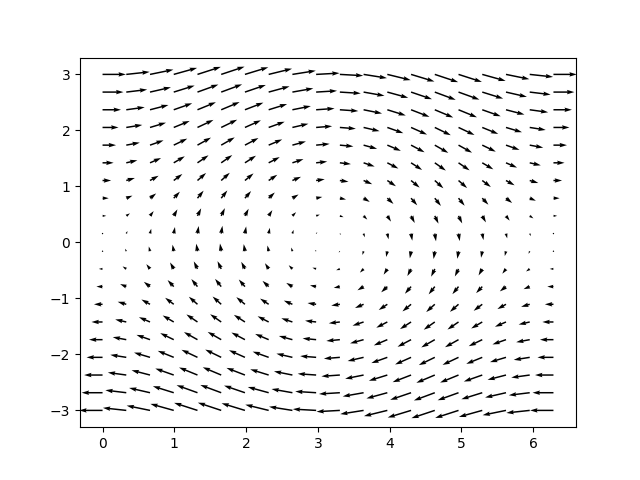
\includegraphics[height=0.7\textheight]{phase_portrait}
\end{frame}

\begin{frame}{Przekroje Poincaré} \pause
Przepływ w N wymiarach $\rightarrow$ Mapa w N-1 wymiarach\\ \pause
W którym miejscu trajektoria znowu przetnie powierzchnię?\\ \pause
\end{frame}

\begin{frame}[fragile]{Przekroje Poincaré - przykład}
\begin{itemize}[<+->]
	\item Weźmy ciało w polu dwóch ciężkich, nieruchomych ciał
	\item Ruch ograniczony do płaszczyzny $(x,y)$
	\item Siła $1/r$ zamiast $1/r^2$
	\item $(x, y, \alpha_v)$ - przestrzeń stanów (po uwzględnieniu $E=\text{const}$)
	\item Przekrój Poincaré dla $y=0$; zaznaczamy punkty $(x, 0, \alpha_v)$ przez które przechodzi trajektoria
\end{itemize} 
\pause
\begin{lstlisting}
./play.py poincare
\end{lstlisting}
\end{frame}

\begin{frame}{Przekroje Poincaré - przykład}
\centering
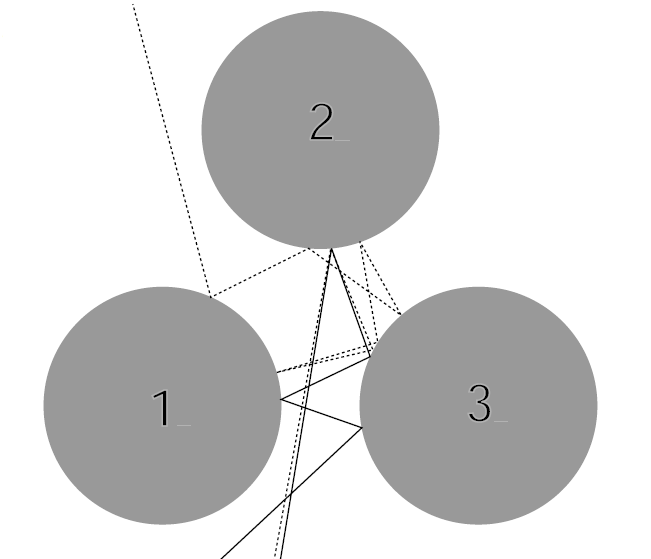
\includegraphics[height=0.7\textheight]{pinball}\\
Każde zderzenie charakteryzuje pozycja i kąt - dwa stopnie swobody\\
Mapa - od jednego zderzenia do kolejnego
\end{frame}

\begin{frame}{Przekroje Poincaré - przykład}
\centering
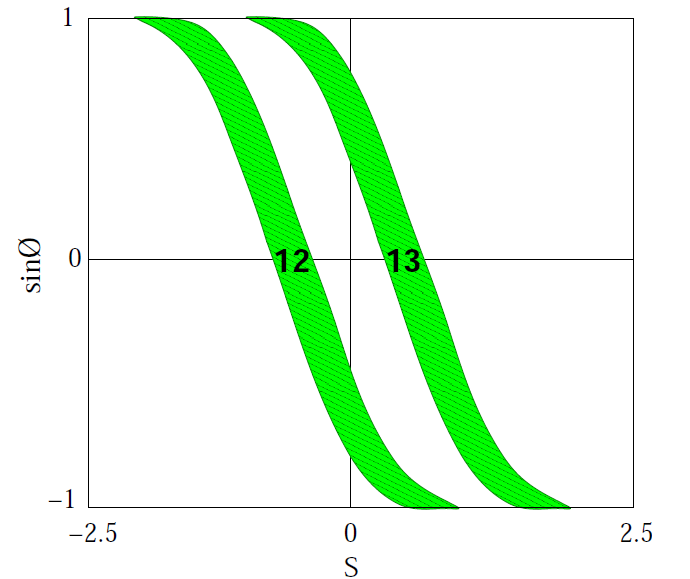
\includegraphics[height=0.7\textheight]{poincare_section}\\
Zielony obszar mapuje się na cały kwadrat w pierwszej iteracji
\end{frame}

\begin{frame}{Entropia metryczna} \pause
	Załóżmy, że mamy odwracalną mapę $M$ na zbiorze $S$.\pause \\
	Chcemy opisać ,,chaotyczność`` $M$ - jak bardzo miesza $S$.\\ \pause
	Zbiór $W$ dzielimy na trzy podzbiory: $\{W_1, W_2, W_3\} = \{W_i\}$.\\\pause
	Wiemy, że w kolejnych $n$ iteracjach mapy punkt $x_0$ trafiał do zbiorów
  $W_{i_1}, W_{i_2}, \dots W_{i_n}$\pause\\
	Co możemy powiedzieć o warunku początkowym $x_0$?\pause
	\begin{equation*}
		x_0 \in W_{i_1} \cap M^{-1}(W_{i_2}) \cap \dots \cap M^{-n+1}(W_{i_n})
	\end{equation*}
\end{frame}

\begin{frame}{Entropia metryczna, cd.}
	\begin{equation*}
		x_0 \in W_{i_1} \cap M^{-1}(W_{i_2}) \cap \dots \cap M^{-n+1}(W_{i_n})
	\end{equation*}
	Jak wiele informacji daje nam ,,symboliczna`` trajektoria $i_1 \dots i_n$?\\ \pause
	$\{W^{(n)}_i\}$ - rodzina $n^3$ zbiorów postaci
	$W_{i_1} \cap M^{-1}(W_{i_2}) \cap \dots \cap M^{-n+1}(W_{i_n})$ \pause \\
	Informacja Shannona:
	\begin{equation*}
		H(\mu, \{W^{(n)}_i\})=\sum_{W \in \{W^{(n)}\}}\mu(W)\ln\frac{1}{\mu(W)}
	\end{equation*}
	$\mu$ - miara probabilistyczna\\ \pause
	Entropia metryczna:
	\begin{equation*}
		h(\mu, M) = \sup_{\{W_i\}}\lim_{n\to\infty}\frac{1}{n}H(\mu, \{W_i^{(n)}\})
	\end{equation*}
\end{frame}

\begin{frame}{Entropia metryczna, cd2.}
	Entropia metryczna:
	\begin{equation*}
		h(\mu, M) = \sup_{\{W_i\}}\lim_{n\to\infty}\frac{1}{n}H(\mu, \{W_i^{(n)}\})
	\end{equation*}
	Fakt: dla dużych $n$: 
	\begin{equation*}
		H(\mu, \{W^{(n)}_i\}) - H(\mu, \{W^{(n)}_i\}) = h(\mu)
	\end{equation*}
 $h(\mu)$ to informacja o $x_0$ jaką dostajemy z każdą kolejną iteracją
\end{frame}

\begin{frame}{Entropia topologiczna}
	Zamiast miary - liczenie zbiorów
	\begin{equation*}
		h_T(M) = \sup_{\{W_i\}}\lim_{n\to\infty}\frac{1}{n}|\{W_i^{(n)}\}|)
	\end{equation*}
	\begin{itemize}
		\item $h_\mu, h_T > 0 $ dla układów chaotycznych i zerowe dla niechaotycznych
		\item Trudne do obliczenia dla rzeczywistych układów
	\end{itemize} 
\end{frame}

\begin{frame}{Epilog - stabilność układu słonecznego}
	\begin{equation*}
	| \delta\mathbf{x}(t) | \approx e^{\lambda t} | \delta \mathbf{x}(0) |
	\end{equation*}
	\pause
	Dla układu słonecznego $\lambda = 1/5\ Myr^{-1}$ \cite{laskar1989numerical}\pause\\
	\textit{In particular, predictability of the orbits of the inner planets, including
	the Earth, is lost within a few tens of millions of years. This does not mean
	that after such a short timespan we will see catastrophic events such as a
	crossing of the orbits of Venus and Earth; but the traditional tools of
	quantitative celestial mechanics (numerical integrations or analytical
	theories), which aim at unique solutions from given initial conditions, will
	fail to predict such events. The problem of the stability of the Solar System
	will have to be set up again, and the qualitative methods initiated by Poincaré
	definitely need to replace quantitative methods in this analysis.}
\end{frame}

\begin{frame}
\nocite{ht_scholarpedia}
\nocite{stewart1994czy}
\nocite{ott2002chaos}
\nocite{ChaosBook}
\bibliography{mybib}{}
\bibliographystyle{plain}
\end{frame}

\begin{frame}[fragile]
Podziękowania
\begin{itemize}
	\item prof. Jakub Tworzydło (IFT)
	\item MP Kolanowski
\end{itemize} 
\pause
\begin{lstlisting}
./play.py stable
\end{lstlisting}
\end{frame}

\end{document}
